\documentclass[14pt , pdftex , hyperref, handout]{beamer} % , notes=show   handout 14pt
\setbeamersize{text margin left=.05cm, text margin right=.1cm}
%\usetheme[height=.8cm, width=0cm, hideothersubsections] {UNLTheme}
\addtobeamertemplate{frametitle}{\vskip-0.2in}{} %move the  title up
  
\usepackage{epstopdf}
\usepackage{natbib}
\usepackage{longtable}
\usepackage{color}
\usepackage{setspace}
\bibpunct{(}{)}{,}{a}{,}{,}
\usepackage{hyperref}   
\usepackage{amssymb}
\usepackage{nameref}
\usepackage{datetime}
\usepackage{ulem}
\newcommand{\cp}[1]{\textcolor{blue}{\scriptsize \citep{#1}}}
\newcommand{\ct}[1]{\textcolor{blue}{\scriptsize \citet{#1}}}
      
%\renewcommand{\ss}[1]{\textcolor{blue}{\small \bf #1}}
\renewcommand{\ss}[1]{{\colorbox{blue}{\color{white}{#1}}}}

\def\newblock{\hskip .11em plus .33em minus .07em}  

\setbeamertemplate{navigation symbols}{} 
\setbeamertemplate 
{footline} 
%{headline}
{\quad\strut\insertsection 
\hfill\insertframenumber/\inserttotalframenumber\strut\quad}

\usepackage[latin1]{inputenc}
\usepackage{tikz}
\usetikzlibrary{shapes,arrows}

\AtBeginSection[]
{
   \begin{frame}
       \ft{\underline{outline}}
\vspace{.2cm}
       \setstretch{.6}\tableofcontents[currentsection]
   \end{frame}
}

\newcommand{\ft}[1]{ \frametitle{ \normalsize \bf{#1}} \vspace{-.4cm}}

\usepackage{colortbl}

\newenvironment{f}[1]
{
  \begin{frame}[fragile,environment=f] 
    \frametitle{ \normalsize \bf{#1}} 
    \vspace{-.4cm} 
    \setbeamercovered{transparent=10} 
    \begin{enumerate}[<+->][$\diamond$]
}{
    \end{enumerate} 
    \setbeamercovered{invisible} 
  \end{frame}
}

\renewcommand{\i}{
\item[$\bullet$] \hspace{-.14in}
}
\newcommand{\s}{
 \item[$\circ$] \hspace{-.14in}
}
\newcommand{\p}{
 \\ \pause
}



\renewcommand{\l}[1]{\small \url{#1}}
\renewcommand{\sl}[1]{\scriptsize \url{#1}}

% a generic beginning
\title{intro}
\author{adam okulicz-kozaryn  \texttt{adam.okulicz.kozaryn@gmail.com}} 
\date{\footnotesize this version: \today \hspace{.2in}\xxivtime} 
\begin{document}
\begin{spacing}{1.2}
\begin{frame}\frametitle{ }
  \titlepage
\end{frame}
\begin{frame}
  \ft{\underline{outline}}
\vspace{.2cm}
\setstretch{.6}\tableofcontents
\end{frame}
% \begin{frame}[allowframebreaks]\scriptsize
% \bibliography{/home/aok/papers/root/tex/ebib}
% \bibliographystyle{/home/aok/papers/root/tex/ecta}
% \end{frame}


% meh not that funny
% \begin{f}{ }\vspace{1.2in}
%   \i \hspace{-.3in} \includegraphics[width=5.1in]{IMG_3152.jpg}
% %  \i \sl{http://www.joearrigo.com/2012/11/30/startling-fact-that-leads-to-better-health-care-at-lower-cost/}
% \end{f}

\begin{f}{ }\vspace{-2.4in}
  \i \hspace{-.3in} \includegraphics[width=4.5in]{IMG_3152.jpg}
%  \i \sl{http://www.joearrigo.com/2012/11/30/startling-fact-that-leads-to-better-health-care-at-lower-cost/}
\end{f}


\section{general overview; approach and policies} %AOK this is strandard %for every class
%LATER see what i have in other classes for intro and standarize it across

% \begin{f}{no food no drink}
%   \i absolutely no food and no drink in the lab!
%   \i use the lounge in the back!!
% \end{f}

% \begin{f}{url}
%   \i you will notice that i heavily use urls
  % \i everything marked with $[*]$ is extra (not required)
  % \i everything marked with ``bonus'' or ``extra'' is not required
  % either
  % \s e.g. if the whole section has ``bonus'' or ``extra'' word -- it
  % is not required
  % \i i add extra things for people who are interested in some specific
  % topics, and want to pursue them farther
 % \end{f}


% \begin{f}{} 
%   \i 
%   % \i urban v rural; city v nature
%   % \i sustainability, natural environment
%   % \i culture,  religion, trust
%   % \i happiness, well-being/quality of life
%   % \i economic and political transition in Eastern Europe
%   % \i programming (Stata, Python)
% \end{f}

\begin{f}{introductions (see if others overlap: can collaborate!)}
  \i about myself \url{http://theaok.github.io}
  \i 
  \i what do you research?
  \s using any data or want to find any data?
  % \s researcher ? what do you research ?
  % \s practitioner ? e.g. what kind of work you do for the county office?
  % % \i programming language (e.g.  stata, python)?
  % \i using any data (e.g. census, GSS)? 
  \i what do you expect from this class?
\end{f}

% \begin{f}{weekly labs; do we need that?}
%   \i find out good time for weekly labs, say Wed 4-5?
%   \i or just 30min before the class
% %  \i email listserv
% \end{f}

\begin{f}{2 keys to success}
  \i start early on ps
  \i ask questions
\end{f}

\begin{f}{approach}
  \i you are encouraged to collaborate (prep for class, ps, paper)
  \i software class! applied, data-driven
%  \i use can usedata that you are working with at yur company
  \i free to choose data/topics as long as relevant to the class
  \s bring your own data; kill 2 birds with one stone
  \s you need to have some data for this class
  \s don't worry, as long as you have any interest, you are likely to
  find data about it
  \s we'll go over data sources in few classes
\end{f}

\begin{f}{before and after the midterm}
  \i 1st half basics, go fast
  \i 2nd half more extras, relax with pace of material but work on paper (final ps/presentation)
  \i before: basics, data, theory, general
  \i after: more specific and advanced topics;  research oriented
\end{f}

% \begin{f}{recommended/extra/bonus}
%   \i e.g.  spatial statistics, online maps,elaborate/complex qgis
%   \s need at least some, you pick depending on what you like
%   \i you will use those additional materials to expand on the basics covered in the class 
%   \p and  enhance your paper 
%   \i I expect, especially PhD students, to read some of the recommended materials 
%   \i note that paper and its presentation is a big chunk of the grade and
%   that's where the additional material matters
% \end{f}


\begin{f}{communication}
 \i email is a preferred mode of communication; just email
 \l {gis\_int@googlegroups.com} 
 \s and everybody in the class
 \s including me and GA will get it
 \s messages will be marked with ``[gis\_int]'' in the subject
 \i you can easily filter them to a specific folder, 
 e.g. in gmail: \sl{http://support.google.com/mail/bin/answer.py?hl=en&answer=6579}
  \i during the  class interrupt me as often as necessary
  \i after the class email me if you have questions -- i
  check email frequently
  \i everyone got welcome email? no? email me
  \i stop by my office!
\end{f}

\begin{f}{ps tips}
  \i \ss{important}: people never follow it
  \i start early
  \i late ps *not* accepted
  \i ask questions early!
  \s do not hesitate to ask questions
  \s there are no ``silly'' questions
  \s it is normal to get stuck and ask questions when learning new software
  \i in class: ask questions / tell me to go slower if needed (i have an impression that i go too fast sometimes)
\end{f}


\begin{f}{class website=syllabus}
  % \i i will be updating syllabus
  % \i the most recent version is always online
  % \i \url{http://aok.mooo.com/gis}
  \i slides are linked from the syllabus
  \i i try to post about a week ahead, but tentative only
  \i print, if you like, right before the class--i am updating continuously
  % \i this is a new class -- i am very happy to get comments/feedback
  % \i let's go over the syllabus
  \i let's see ps directions %and esp wiki
\end{f}


% \begin{f}{files}
%   \i never send me anything in word format
%   \i files names must not have spaces
%   \i for big files use something like dropbox and give me the link
%   \i do not double-zip (zipped file in a zipped file)
%   \i per url's give exact addresses, not just generic (e.g. http://census.gov)
%   \i i will be picky about it
% \end{f}

% \begin{f}{text file/ascii}
%   \i it is NOT .doc .rtf or .odt
%   \i it is plain text
%   \i to check if it is plain text, open it in notepad
% \end{f}

%\section{this class specifically}


% \begin{f}{the difference}
%   \i this class is different from other classes
%   \i fundamentally this class is about software
%   \s and hands-on, applied, usage of it
%   \i it is impossible for me to cover everything that you may bump
%   into
%   \i that's why it is key for us to communicate well
%   \s don't hesitate asking the questions
%   \s use email extensively (eg couple times per day)
% \end{f}

% \begin{f}{general vs specific}
%   \i i will be rather focused on general themes rather than specific
%   \p less talk about zoning, highways; more about data formats;
%   general geographic laws
%   \p in short, more research and hands-on application, fewer specifics
%   \s e.g. ``positive spatial autocorrelation'' is such a general theme
%   \s e.g. ``zoning in Camden'' is a specific theme
% \end{f}


% \begin{f}{geography and levels}
%   \i U/As are always nested...
%   \i e.g. state-county-city-street
%   \p (still, keep in mind that not always the whole is a simple sum of
%   parts)
%   \p we will discuss it later, the so called atomistic and ecological
%   fallacies
%   \p idea is simple:
%   \i Rutgers is a good university, hence you are good students
%   \i you are good students, hence Rutgers is a good university...
% \end{f}

% \begin{f}{research vs practice}
%   \i i am a researcher, not a practitioner
%   \i researchers are academics, PhD students...
%   \i practitioners are government officers, MPA students
%   \i there is a big difference between researchers and practitioners
%   \s yet, practice should be based on research
%   \s and research should result in improvements of the practice
%   \i practitioners should read some research
%   \i researchers should be familiar with the practice...
% \end{f}

\section{why?}

\begin{f}{a general thought about maps}
  \i maps are always useful
  \i no matter what you study it always takes place somewhere and place matters
  \i so you should use maps for whatever you study in *all* other classes
  \i and all other projects outside of school
  \i it will always help with understanding of what is going on
  % \i and it is not that difficult!
  % \i most of you are already at stage where you produce great maps!
\end{f}

% \begin{f}{so what? geography matters!}
%   \i with maps you get insight you won't get otherwhise
%   \i oftentimes all you have to do is to map it
%   \s and think \textbf{a lot} about what you have mapped 
%   \s and what it really means
%   \s eg Dick De Veaux: faulty devices around Rocky Mountains 
%   \s eg Cooper's Hospital dr Brenner:  ER visits home addr
%   \s send nurses to homes and cut costs dramatically and improve health %(i think!, correct me if i am wrong!)
% % \sl{https://www.camdenhealth.org/dr-brenner-discusses-the-nations-healthcare-system/}
% % \s \sl{http://www.rwjf.org/en/library/articles-and-news/2014/02/improving-management-of-health-care-superutilizers.html}
% \end{f}

% \begin{f}{why? discovery! just put it on a map}
%   \i  Dick De Veaux: \ss{blackboard:} US map with loc of faulty devices
%   \i and Cooper's dr Brenner on next slide
% \end{f}

\begin{f}{ }
  \i \vspace{-.1in} 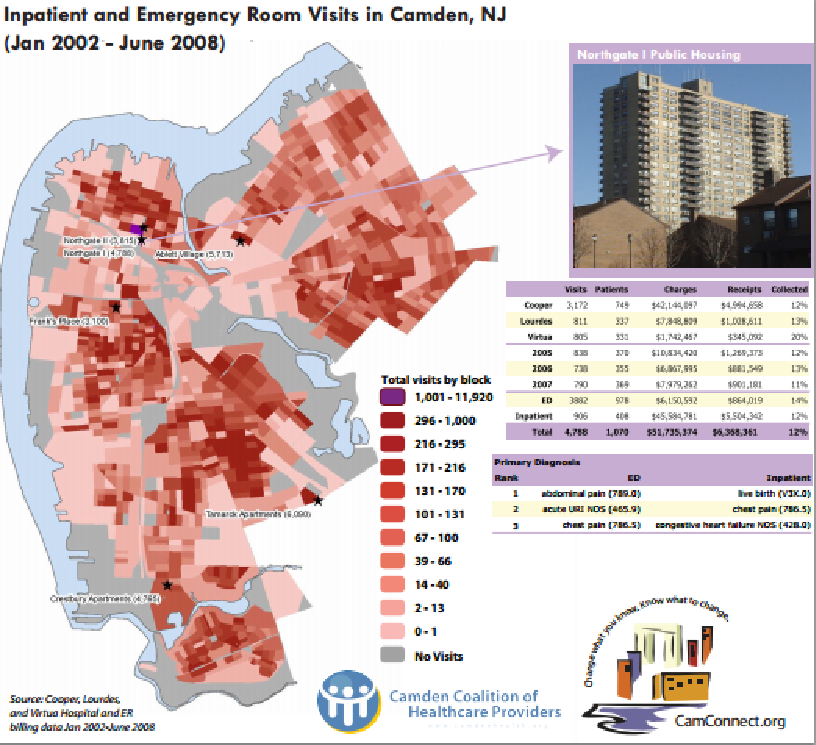
\includegraphics[width=4.4in]{art-camden.pdf}
%  \i \sl{http://www.joearrigo.com/2012/11/30/startling-fact-that-leads-to-better-health-care-at-lower-cost/}
\end{f}

\section{what is GIS?} %briggs_intro/fund.ppt

\begin{f}{what is there?}
  \i GIS Geographic Information Systems
  \s Geographic: Cities, Roads, Rivers, Countries, etc
  \s Information Systems: data, software, programming,   
  \s like MIS (Management Information Systems) or IT
  \i GIS=CS(graphics, database/sys adm, coding)+geography
  \i really, much of the GIS is data management 
  \i geographic$=$geospatial$=$spatial (synonymous)
\end{f}

\begin{f}{past and future}
  \i much of the gis has been (still is) done with ArcGIS/ArcMap
  \s this is more of a dinosaur, however
  \i the future is open source software like QGIS
  \i and internet companies like Google
\end{f}

\begin{f}{what we'll be doing}
  \i obtain (download, but also eg smartphone/gps), manage and display data
  \s a display is usually a map
  \s really, this class is mostly about producing maps
  % \i we will calculate simple spatial statistics
  % \s in the second part of the class (bonus)
  \i there is much more to the GIS, of course
  \i this class is just applied mapping
\end{f}

\begin{f}{maps}
%  \i much of the class is about maps
  \s keep in mind that a map is visual representation of data
  \i there is always a database behind a map
  \s (database is like spreadsheet, but bigger and fancier)
  \i or more precisely: 
  \s there is sometimes a map on the top of the database
  \s so maps is just data in the picture
  \i the bottom line is data !
\end{f}

\begin{f}{why GIS in social science?}
  \i local government 
  \s zoning, public works (streets, water supply, sewers), garbage
  collection, land ownership and valuation, public safety (fire and police)
  \i federal/state
  \s natural resource management
  \s highways and transportation
  \i any academics:  ``no matter what you study it takes place somewhere''
   (place always matter)
  \s perhaps esp public health/epidemiology and criminology 
\end{f}

\begin{f}{why GIS?}
  \i businesses
  \s retail site selection \& customer analysis
  \s logistics: vehicle tracking \& routing
  \s natural resource exploration (petroleum, etc.)
  \s civil engineering/construction
  \i so you see that you can do a lot with GIS
  \i yes, it gives you specific, marketable job skills
%  \s an unlikely combination for a soc sci class
\end{f}

\begin{f}{ext cre opport $\le$10\% of final grade; harsh grading!}
  % \i present your final project early 
  % \s in addition to extra credit you will get feedback how to improve it
  % \s and you have to do it anyway later
  \i present sth not covered (has to be GIS, of course)
  \i present alternative way of doing sth that we have covered
  \i civic engagement: check out these,
  and email listserv by ext week which one you'd like to do
  % Michael D'Italia michael.ditalia@camden.rutgers.edu
  % LATER add to syllabus, guess just copy from                                %research meth or qm2...
  \i \url{https://cpachvi.org/about/homeless-services/}: SJ: homeless, poverty 
  \i \url{http://www.laeda.com}: camden small businesses
  \i \url{https://rand.camden.rutgers}: SJ: health, etc % talk to Darren or Sarah \url{https://rand.camden.rutgers.edu/people/staff/}
  \i \url{virtua.org}: SJ: health %talk to Lisa LRosenberry@virtua.org  \url{https://www.linkedin.com/in/lisa-rosenberry-7331904b}
\end{f}


\begin{f}{maps are fun! (\textbf{at the end if time!}}
  \i let's look at some interesting maps
  % \i you'll see that mapping can be useful 
  \s see patterns that cannot see otherwise 
  \s absorb easily lots of information
  \s compare easily
%  \i examples are supposed to inspire you to produce your own maps
  \i \l{https://digg.com/2020/which-state-hates-which-state-map}
  % ALT: https://www.instagram.com/p/B7bkVkZnogM/?utm_source=ig_embed
\end{f}

% \begin{f}{examples}
%   \i election results (just goog img)
%   \i spread of diseases
%   \i weather map/radar
%   \i housing prices (trulia, zillow)
% \end{f}

% \begin{f}{acs}
%   \i American Community Survey (acs) is a great source of regular and gis data
%   \p \l{http://www.census.gov/acs/www/data_documentation/2009_acs_maps/}
%   \p let's see the following by county
%   \s \% foreign born 
%   \s mean travel to work
%   \s completed hs;  have bs/ba
%   \s below poverty level
%   \s housing value
% \end{f}



\begin{f}{the big sort}
  \i ``The  big sort 
  \p why clustering of like-minded America is tearing us apart''
  \i America polarizes by county
  \p (counties are becoming either R or D)
  \i \l{http://www.thebigsort.com/maps.php}
\end{f}

\begin{f}{who is your city}
%  \i just google ``who is your city''
%  \l{http://utd.edu/~ajo021000/myweb/other.html}
  \i \l{http://www.creativeclass.com/_v3/whos_your_city/maps}
\end{f}

% \section{[skip, nobody likes it] qgis on apps.rutgers }

% \begin{f}{server/cloud}
%   \i  we will try to use apps.rutgers
%   \i why bother with this?
%   \i this is the future, in 10 years everybody will use it
%   \s so you may get used to it now
%   \i and a part of data management is to use a remote server
%   \s again GIS$\approx$data management
%   \i faster, more reliable, accessible from anywhere, persistent sessions
%   \i but you can run it on any pc, any OS
% \end{f}

% \begin{f}{today}
%   \i first, the difficult part
%   \s connect to apps.rutgers
% \end{f}

% \begin{f}{we'll work on apps}
%   \i make sure you have it enabled
%   \i go to \url{http://netid.rutgers.edu/}
%   \i on the left, click ``service activation''
%   \i and activate ``apps cloud service''
% \end{f}

% \begin{f}{connect to apps.rutgers}
%   \i Either go to \url{https://apps.rutgers.edu} or \url{https://apps.rutgers.edu/novnc/} (clunkier, but works on tablets)
%   \i To copy files, you can either \url{https://apps.rutgers.edu} 
%   \i For a nicer interface install \url{http://winscp.net/}, run it
%   and connect to: Host name: "apps.rutgers.edu"; User name: "your
%   Rutgers NetID"; Password: "your Rutgers password"
% \end{f}

% \begin{f}{but you can just use your PC}
%   \i QGIS is open-source
%   \i just google it...
%   \i then you can brig your own laptop and work there...
% \end{f}


\end{spacing}
\end{document}

